\documentclass[letter, USenglish, 11pt, subfigure]{article}
\usepackage[margin=1in]{geometry}
\newcommand*{\ATLASLATEXPATH}{./}
\usepackage{\ATLASLATEXPATH atlaspackage}
\usepackage{\ATLASLATEXPATH atlasbiblatex}
\usepackage{\ATLASLATEXPATH atlasphysics}
\usepackage{\ATLASLATEXPATH ANA-SUSY-2018-12-PAPER-defs}
\usepackage{enumerate}
\usepackage{caption, float, threeparttable}
\newcommand{\tth}{\ensuremath{\ttbar H}}
\newcommand{\ttH}{\ensuremath{\ttbar H}}
\newcommand{\tthyy}{\ensuremath{\ttbar H(\to\gamma\gamma)}}
\newcommand{\myy}{\ensuremath{m_{\gamma\gamma}}}
\newcommand{\hyy}{\ensuremath{H(\to\gamma\gamma)}}

\usepackage{lineno}
\usepackage{titlesec}

%\linenumbers
\usepackage{wrapfig}
\usepackage{placeins}
\usepackage{pdfpages}
\usepackage[none]{hyphenat}

\usepackage{xifthen}
\usepackage{multirow,bigdelim,makecell}
\usepackage{cellspace}
\usepackage{selectp}
\usepackage{color, colortbl}

% \outputonly{1}
\usepackage[nottoc,numbib]{tocbibind}

\addbibresource{proposal_WHopkins.bib}
\addbibresource{ATLAS-SUSY.bib}
\addbibresource{ATLAS.bib}
\addbibresource{ANA-HDBS-2021-10-PAPER.bib}
\addbibresource{CMS.bib}

\pagestyle{headings}

\title{Early Career Research Proposal: \\Enabling Calibrations of Machine Learning Approaches (ECMLA)}
\author{Applicant/Institution: Walter Hopkins, Argonne National Laboratory\\ Postal Address: \\Argonne National Laboratory, 9700 S. Cass Avenue, Building 360, Lemont, IL 60439
  \\PI name: Walter Hopkins\\Position title for PI: Physicist\\PI telephone number, email: (630) 252 7551, whopkins@anl.gov\\Administrative Point of Contact name, telephone number, email:\\Diane Hart, (630) 252 7677, dhart@anl.gov\\FOA Number: DE-FOA-0003176\\DOE/SC Program Office: HEP\\ Topic Area: Experimental Research at the \\Energy Frontier in High Energy Physics\\DOE/SC Program Office Technical Contact: Abid Patwa\\Year Doctorate Awarded: 2013\\Eligibility Extension Included in Approved Pre-application: No\\Does the PI have tenure: No\\Number of Times Previously Applied: 2\\PAMS Pre-application Number: PARE-0000036282\\PECASE Eligible: Yes\\Proposal Contains Data Management Plan in Appendix 4: Yes\\Proposal Contains PIER Plan in Appendix 5: Yes
}
\date{}

\begin{document}
\pagenumbering{gobble}

% Play up that these are tricky ML techniques to implement and you have a goal of removing barriers to more wide spread use across HEP 
% * i still don't understand what SALT does. you could explain it more
% * i'm not sure decorrelating ID vs track isolation is critical. as we've discussed, there are other ways to calibrate such as disco or things that give two decorrelated outputs. in that case you could literally use isolation as an input
% * motivate tth more. it's exciting physics - why? 
% * re: tth you could do more here, for example mentioning the system reconstruction. you can tie that to work with gretel. or not. but right now the system reconstruction is done using 4vectors and BDTs. ugh
% * i tried to read careful and struggled to understand what feature transfer does
% * can the two tth analyses be split a bit more so they don't sound so similar? or to add more physics motivation?
% 

\maketitle
\clearpage
\tableofcontents
\thispagestyle{empty}

\clearpage
\pagenumbering{arabic} 
\section{Introduction}

Experiments at the Large Hadron Collider (LHC) have confirmed many predictions of the highly successful Standard Model (SM), including the landmark discovery of the Higgs boson~\cite{HIGG-2012-27,CMS-HIG-12-028}. Despite its success, the SM does not account for several observed phenomena, such as dark matter and the matter-antimatter asymmetry, thereby fueling the search for Beyond the Standard Model (BSM) physics. Future LHC upgrades will shift focus from increasing energy to enhancing precision, marked by a tenfold expansion of the Run~2 dataset in the High Luminosity-LHC (HL-LHC) phase. Crucially, enhancing the efficiency of measurements and minimizing systematic uncertainties are vital for future breakthroughs in collider physics. Increased efficiency effectively increases the usable data, akin to extending LHC operation times, while reducing systematic uncertainties further heightens the sensitivity to subtle deviations from SM predictions.

Machine learning (ML) has increasingly become a critical tool in High-Energy Physics (HEP), offering significant advancements in various tasks such as identifying particles and distinguishing between signal and background processes. ML techniques allow physicists to leverage complex correlations among a wide range of observables, from the trajectories and energies of particles to their interactions within detectors. However, the application of ML in HEP is accompanied by certain challenges that need careful consideration: 1) Sensitivity of ML models to differences between Monte Carlo simulations and recorded data, which can introduce additional uncertainties into ML predictions and affect the overall systematic uncertainties in physics measurements; 2) Sensitivity of ML algorithms to experimental parameters (e.g., the energy resolution of a subdetector) which increase systematic uncertainties in the final result; 3) Tendency of ML models to sometimes create unintended correlations between their outputs (such as particle identification) and other variables critical for calibrations or background estimations.

Recent applications of adversarial~\cite{louppe2017learning} and distance correlation~\cite{PhysRevLett.125.122001} techniques have shown promise in reducing uncertainties due to data-simulation differences in a long-lived particle search~\cite{calRatio} and in decorrelating jet substructure variables from jet mass~\cite{ATL-PHYS-PUB-2018-014}. These approaches are part of a group of methods that aim to improve the 'domain adaptation' of ML algorithms, i.e., the ability of an ML model trained with one dataset (e.g., simulations) to be robust enough to yield similar performance on a different dataset with somewhat different features. This robustness can be achieved in several ways, for example, by including the alternative dataset during training and penalizing differences in performance.

domain-adaptation techniques can enhance the resilience of ML models used in HEP against data-simulation discrepancies, varying detector and accelerator conditions (e.g., the number of simultaneous proton-proton interactions, known as pile-up), and changes in the underlying parameters of simulations, such as those used for estimating the properties of physics objects (e.g., photon energy, jet transverse momentum, etc). These techniques also aid in identifying (ID) physics objects (e.g., photons, jets containing $b$-hadrons, etc). Thus, incorporating domain adaptation into the HEP ML workflow can significantly reduce the overall uncertainties in physics results.

This proposal {\textbf outlines the development of a framework designed to facilitate the deployment of various domain-adaptation techniques within existing and future HEP ML workflows. This framework is intended to enhance the resilience of ML models against experimental systematic uncertainties, data-simulation discrepancies, and changes in detector or collider conditions, which will subsequently reduce uncertainties and thus improve the discovery potential of the HL-LHC.} Given recent initiatives within HEP to adapt ML models for use with field-programmable gate arrays (FPGAs), the proposed framework will also improve ML models deployed at the trigger level. Moreover, the PI's team will introduce a novel domain adaptation method to HEP, termed ``feature representation transfer.'' This method is designed to generate robust, generally applicable features—such as those usable for both particle identification and energy determination—unlike the currently utilized methods of distance correlation and adversarial networks, which tend to be more application-specific (even within similar applications such as particle ID and energy determination).

Precise measurements of SM processes, particularly those involving Higgs bosons, play a crucial role in probing for BSM effects caused by particles too massive to be directly produced at the LHC. Higgs differential cross-section measurements, i.e., as a function of kinematic properties such as Higgs \pt, are critical probes for BSM physics because they are sensitive to deviations in the Higgs boson self-coupling and its coupling to the top quark. The latest ATLAS \hyy\ differential cross-section measurements, which include the associated production of a Higgs with a top pair (\tth), are limited by statistical uncertainties in each kinematic bin. Enhancing object ID efficiencies, especially for photons which improves the statistical power of the measurement, and reducing dominant detector-based systematic uncertainties, such as photon ID and energy resolution, are crucial for improving these measurements and thereby maximizing sensitivity to BSM physics.

The proposed framework and techniques will initially be developed and applied to photon ID and energy. Studies within ATLAS have shown a potential improvement of approximately 10-20\% in both ID efficiency (equivalent to collecting more data) and energy resolution when all available information for ID and energy calibration is included. However, once calibration—a process that involves evaluating ID efficiencies and properties in simulations and adjusting them to match true properties before reconstruction or to match observed data, the gains in efficiency and enhancement in resolution were lost. For the ID, ML approaches were found to correlate with quantities that must remain independent of the ID for the calibration method, while for energy determination, ML methods were sensitive to mis-modeling of shower shapes in the simulation. Therefore, the proposed domain adaptation framework and approaches could enhance all ATLAS measurements involving \hyy, which are vital to the HL-LHC BSM search program.

As collider physics enters the precision era and ML becomes increasingly integral to our methodologies, it is crucial to refine ML models to achieve heightened precision in anticipation of the HL-LHC startup. The PI's extensive background in ML, demonstrated through leadership roles such as convening the ATLAS ML Forum and co-developing a novel feature extraction technique~\cite{dijetAnom}, aligns perfectly with the goals of this project. Additionally, the PI's deep experience with calorimetry and simulations, combined with the PI's involvement in prominent searches involving $\ttbar$ final states and recent analyses using two-photon final states, equips me uniquely to lead the proposed research.

At Argonne the advanced computing resources that have supported substantial ATLAS group analyses and ML initiatives present a distinct advantage. These facilities will play a critical role in developing and implementing the proposed ML framework. This convergence of timing, expertise, and resources at Argonne makes it the ideal moment and place for this essential research. By advancing ML techniques now, we can ensure that the HL-LHC's full potential for discovery is realized.

\clearpage

\subsection{Limitations of Differential Cross-Section Measurements at the HL-LHC: Uncertainties}
The HL-LHC will deliver a vast HEP dataset providing opportunities to perform new measurements and with unprecedented precision.
Many measurements which were statistically constrained will become limited by systematic uncertainties which underscores the pivotal role of systematic uncertainties in shaping the landscape of precision measurements within the HEP. There are, however, measurements with potentially significant BSM contributions that will benefit from an even greater increase of the dataset size. Such an increase is only possible by improving the ID efficiency of physics objects that are expected to be present in various final states. 

Measurements involving the SM Higgs become increasingly sensitive to high mass BSM contributions as the precision of measurements improves. As the size of the LHC dataset grows, differential cross-section measurements, which can further expose the effects of BSM physics in high-energy regions (see Figure~\ref{fig:SMEFT_highmass} for an illustration of this effect), become more powerful tools in the search for BSM physics. The results of differential cross-section measurements can probe BSM effects by being interpreted in the context of the Standard Model Effective Field Theory (SMEFT)~\cite{Buchmuller:1985jz,Grzadkowski:2010es,SMEFTsim3} and in the case of Higgs-related measurements, results can also be interpreted in terms of coupling strengths within the $\kappa$-framework~\cite{deFlorian:2016spz}.

\begin{wrapfigure}{r}{0.6\textwidth}
  \centering
  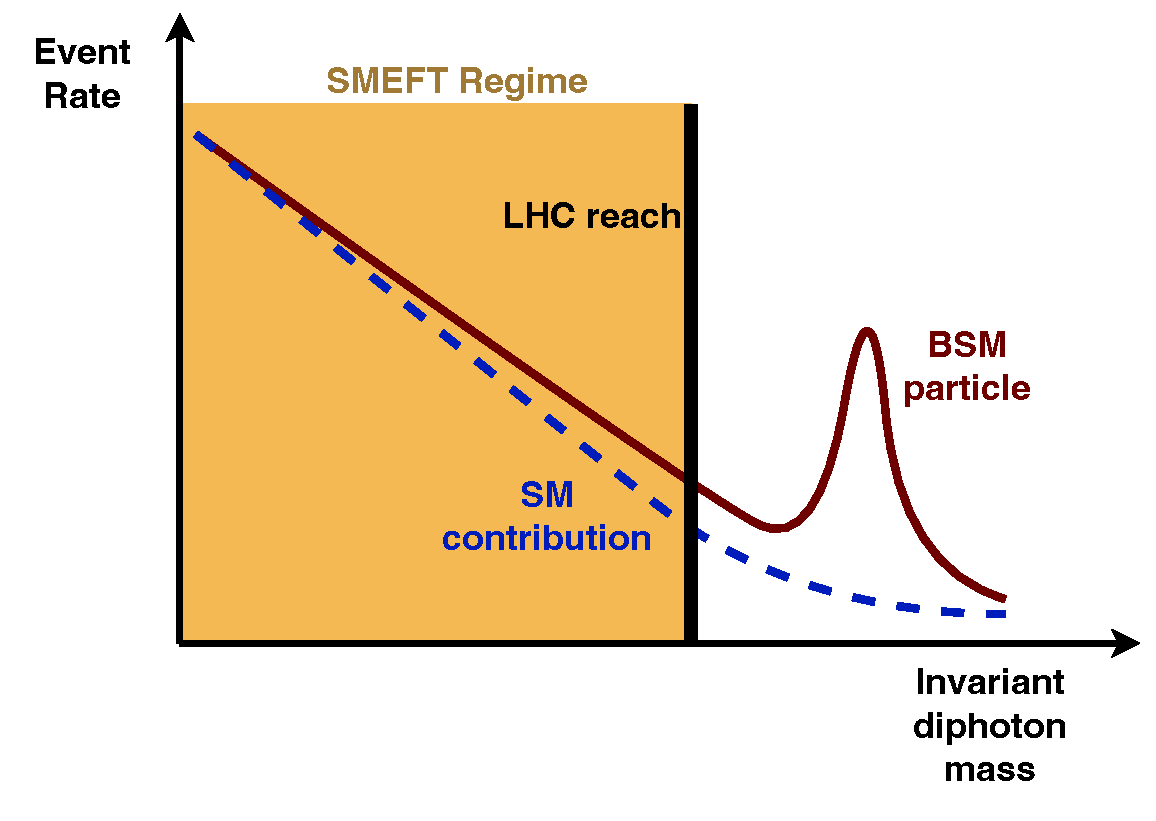
\includegraphics[width=\linewidth]{figures/SMEFT.pdf}
  \caption{\label{fig:SMEFT_highmass} Example of how effects of a heavy BSM particle can leak into high-energy regions of distributions measured at LHC experiments.}
\end{wrapfigure}

A recent differential cross-section measurement involving the decay of the SM Higgs to two photons~\cite{ATLAS_STXS} utilized the Simplified Template Cross Section (STXS) method. This approach measures cross-sections in bins across several kinematic dimensions to constrain BSM effects via the SMEFT interpretation. Although current measurements are statistically limited and suffer from substantial systematic uncertainties - up to approximately 40\% in some differential cross-section bins - the HL-LHC's larger dataset will mitigate statistical limitations in most bins, thus amplifying the significance of reducing systematic uncertainties. However, bins in high-energy regions, such as those measuring properties of a Higgs produced in association with a top pair (\tth), will still face statistical limitations. Improving photon ID efficiency could reduce statistical uncertainties by up to 17\% in final states that include two photons. This improvement requires ensuring that photon ID is uncorrelated with track isolation. The methods, such as distance correlation and adversarial techniques, incorporated into the proposed framework can be applied to a new ML-based photon ID algorithm to achieve increased statistical power in topologies with two photons.

\subsection{Reducing Uncertainties with an ML Domain Adaptation Framework}
Machine learning has been utilized for the identification of various physics objects, such as electrons and jets containing b-hadrons. However, many of these ML models rely on simulations for training and do not automatically account for data-simulation differences during this phase—this issue is typically addressed during calibration. Furthermore, algorithms may need to remain independent from variables that are part of the calibration process, for example, those used to determine the rate of fake objects~\cite{atlas_photon_id}, or variables that may vary during collider or detector operations, such as pile-up. Enhancing the robustness of ML models used to identify objects and assess their properties—thus mitigating these effects—will have far-reaching impacts on physics results.

There have been recent advancements in using domain-adaptation techniques to decorrelate ML models from certain quantities using methods such as adversarial discriminants and distance correlation. Adversarial approaches involve two ML models, one that generates high-dimensional distributions and another model that is trained to discriminate between the ML-generated data and the real data. More recently, adversarial approaches have been used to discriminate between recorded and simulated data from the output of another discriminator~\cite{calRatio}. This strategy, i.e., to impose penalties on an ML model for producing inconsistent results across various datasets, can be applied to minimize differences between data and simulations or between simulation datasets with different parameter values (e.g., the energy resolution of jets). This is achieved by including two optimization quantities (i.e., cost or loss functions), one for each ML model. Using two opposing ML models to improve domain adaptations allows for complex multi-dimensional correlation to be taken into account. However, this dual-faceted optimization process introduces a significant computational demand and presents challenges in establishing definitive criteria for the cessation of training.

An alternative method that easier to implement but may not be able to take advantage of as much information as adversarial approaches, is using distance correlation which summarizes the dependence of sets of variables. Unlike the more frequently used measure of the Pearson correlation coefficient, which can only detect linear correlations, distance correlation is sensitive to non-linear correlations, which are commonly present in HEP datasets. The distance correlation is zero only and only if there are no correlations between the input variables. This feature allows it to easily be added to typical loss functions which are minimized to optimize ML models. Thus, distance correlation is simpler to implement than adversarial techniques with less hyperparameters (since only a loss term is added rather than an entire NN) and more stable training characteristics. 
\begin{wrapfigure}{L}{0.55\textwidth}
  \centering
  \includegraphics[width=\linewidth]{figures/framework.pdf}
  \caption{\label{fig:framework} Sketch of the proposed framework. The pink box and arrow highlight the new parts of ML training workflows. The ``true value of target'' represents known quantities in the simulations such as the event classification (signal vs background), object identification (real photon vs fake), or a quantity such as the true energy of a photon before it is measured by a detector. }
\end{wrapfigure}
Another, less explored within HEP, domain adaptation technique is feature representation transfer. The idea is to learn a feature representation that is domain-invariant. Techniques such as autoencoders networks (which take inputs and encode them into a lower-dimensional space) can be used to learn such representations where the model minimizes the difference between the source (e.g., simulation) and target (e.g., recorded data) domain features, making the model's predictions less dependent on the domain-specific features. The advantage of feature representation transfer over distance correlation and the adversarial techniques is that the resulting domain-adaptive features can be used for a variety of tasks. These features would be akin to physicist developed variables that are ratios of quantities that behave similar after a change in assumption (e.g., both the numerator and denominator increase at a similar scale if an energy scale is changed).

\begin{table}
  \caption{\label{tab:methods}Domain-adaptation techniques that will be studied and applied to various tasks detailed in this proposal. }
  \begin{tabular}{|l|c|c|c|} \hline
    {\textbf Method} & {\textbf Maturity in HEP} & {\textbf Main Benefit} & {\textbf Compute Intensity} \\  \hline\hline 
    Adversarial & used & complex correlations & high \\ \hline
    Distance Correlation & used & non-linear correlations & low \\ \hline
    Feature Transfer & not used & features for multiple tasks  & medium \\ \hline\hline                                                                                                                                       
  \end{tabular}
\end{table}

Domain adaptation allows ML models to maximize the use of all information while avoiding regions of kinematic phase space that are poorly modelled in simulation or to ensure an ML model is independent of a quantity, such as pile-up or isolation. Depending on the particular application, adversarial, autoencoder based feature representation transfer, or distance correlation approaches can be the optimal solution and all should be studied when developing a particular ML model. A summary of the approaches that will be developed and applied are listed in \cref{tab:methods}.

Recently, ML frameworks have been developed that are capable of training regression or classification models. These frameworks are multi-modal, meaning they can handle various types of input data (such as particle trajectories and jets), and multi-task, allowing them to build complex ML models for a range of tasks (such as identifying jets containing hadrons initiated by charm or bottom quarks, and performing jet energy corrections). SALT~\cite{salt}, a framework developed within ATLAS but not limited to ATLAS applications, exemplifies such a system. It can identify objects and separate signal from background processes using different types of data. While these frameworks are powerful tools, they often lack the infrastructure needed to automatically produce models that are robust against simulation mismodeling, experimental systematic uncertainties, or pile-up (see \cref{fig:framework} for a depiction of how domain adaptation fits into the current training paradigms). Incorporating domain-adaptation techniques within SALT will help reduce systematic uncertainties, benefiting many physics results. %Finally, the rise of ML-focused High-Performance Computers (HPCs), such as Aurora at the ALCF, are an opportunity to deploy these domain-adaptation approaches, which can be compute intensive, across applications in HEP.

\subsection{Initial Uses of Domain Adaptation: Photon ID and Energy Determination}

Improvements in photon energy calibration have been studied using advanced ML architectures, such as convolutional neural networks (CNNs) and graph neural networks (GNNs), and by providing more information to the current BDT-based algorithm. The preliminary results of this ML-based energy determination showed a $\sim$20\% improvement in photon energy resolution but was sensitive to simulation mismodelling in variables that summarized the shape of the energy deposits in the calorimeter. Ensuring that ML models are insensitive to the observed mismodelling in certain corners of the dataset could result in significantly improved photon energy resolution which in turn will reduce the systematic uncertainties for analyses that include photons in their final states (which includes all channels that involve \hyy\ decays such as the Higgs mass measurement).

Machine-learning-based photon ID techniques (i.e., a boosted-decision-tree, BDT) have been studied within ATLAS demonstrating a potential gain in signal efficiency of 5-10\% (e.g., moving from 88\% to 95\% efficiency for unconverted photons with \pt$\sim$60 GeV) resulting in an increase of statistics of 10-20\% (thus reducing the statistical uncertainty by 10-17\% for events with two photons) while retaining the same background rejections as the current rectangular-requirement-based ID. An increase in efficiency would impact all \hyy\  measurements by improving the statistical power of these measurements with the same amount of HL-LHC data while increasing the background rejection (once the signal efficiency has saturated) will result in an even purer \hyy\  signal. Even more efficiency gains and increased background rejection have been observed when using CNNs. However, photon ID calibration procedures and fake-photon background estimation techniques used in many ATLAS analyses necessitate that the photon ID remains uncorrelated with track isolation (a measure of the energy associated with the photon candidate versus the energy around the candidate). This requirement for orthogonality to specific quantities has limited the use of ML for photon ID within ATLAS. Additionally, the Phase II upgrade of the ATLAS Inner Tracker (ITk) presents an opportunity to revisit the ATLAS photon ID and its calibration to maximize performance during the HL-LHC.

\section{Project Objectives}

The goal of this proposal is to significantly enhance the discovery potential of the HL-LHC by both augmenting the statistical power of measurements and reducing the impact of systematic uncertainties on precision measurements via the integration of domain-adaptation techniques into ML models. Initially, domain adaptation will be applied to the ATLAS photon ID and energy determination, which will subsequently be utilized in the upcoming \hyy\ differential cross-section measurements. Moreover, these domain-adaptation techniques will refine the signal-versus-background discriminant in the \hyy\ measurement. The resulting ML framework will provide streamlined access to domain-adaptation techniques that not only automatically counteract systematic uncertainties but also simplify calibration tasks, such as adjusting simulations to align more closely with recorded data, across a broad spectrum of applications within HEP.

\begin{itemize}  
\item \textbf{Develop an Integrated ML Domain-Adaptation Framework}
  \begin{itemize}
  \item Construct a framework that seamlessly incorporates domain-adaptation techniques during the development of ML models, ensuring robustness and adaptability
  \end{itemize}

\item \textbf{Deploy Domain Adaptation Techniques}
  \begin{itemize}
  \item Improve photon ID and energy calibration using domain adaptation
  \end{itemize}
  
\item \textbf{Improve Run~3 \hyy\ Differential Cross-Section Measurements with Domain Adaptation}
  \begin{itemize}
  \item Use domain-adaptive photon ID and energy determination to improve the \hyy\ differential cross-section measurement
  \item Apply domain-adaptation techniques to improve discrimination between signal and background processes in the \hyy\ differential cross-section analysis
  \end{itemize}
\end{itemize}

\clearpage

\section{Proposed Research and Method}

The PI's team will customize and deploy domain-adaptation techniques within an ATLAS common framework, i.e., ``SALT''~\cite{salt}. These techniques will first be applied to improve photon energy determination and photon ID. The more established approaches, distance correlation and adversarial networks, will be studied in parallel with feature representation transfer. 

Domain-adaptation techniques will first be applied in conjunction with BDTs and will then be adapted to be used with more advanced networks such as GNNs. The adversarial approaches as well as GNNs require significant computing resources to train and tune. The PI will leverage both computing resources and expertise at Argonne to develop domain adaptive models.
The team will assess the effectiveness of domain-adaptation techniques by examining residual correlations and comparing the performance of ML models with and without domain adaptation. Upon successful validation and integration of these techniques into SALT, the PI's team will with members of the Argonne ATLAS group (who will not be funded by this proposal, if awarded), who are working within the ATLAS flavor tagging group, to implement the domain-adaptation approaches for flavor tagging.

In parallel to preparing domain adaptation for use in ATLAS physics object ID and property determination, the PI's team will contribute to two differential cross-section measurements of \hyy: an intermediate analysis using a subset of Run 3 data, and a comprehensive final result utilizing the entire dataset. The improved photon energy determination and ID calibrations will be used with the full Run 3 \hyy\  measurement. The PI's team will focus on ensuring that the MVA used for signal-background separation does not sculpt the diphoton mass (an essential ingredient to the background estimation) which will benefit measurements in all the bins of this diifferential cross section measurement. The PI's team will focus on the \tth\ measurement drawing from previous experience with final states that include $\ttbar$ within Supersymmetry searches and more recently, final states that include two photons within a charged Higgs search. 

\subsection{Reducing the Effect of Simulation Mismodelling in Photon-Energy Determination with Domain Adaptation}

The calibration of photon and electron energy involves several steps as detailed in~\cite{atlascollaboration2023electron}. This proposal aims to test and enhance the simulation-based calibration that utilizes variables derived from energy deposits grouped in the calorimeter. The process aims to adjust for energy that is lost in material before the calorimeter, deposited in adjacent cells, or not captured by the LAr calorimeter. The current algorithm uses a BDT to regress the corrected photon energy using shower-related variables that summarize shower properties (see Figure~\ref{fig:showerVars}). The BDT is trained with a single particle simulation with a flat transverse momentum (\pt) spectrum up to 150 GeV. The performance of the BDT is then evaluated by comparing the energy predicted by the BDT with the true particle energy. Internal ATLAS studies have shown that adding lateral shower shape variables to the BDT could improve the energy resolution after calibration by 10-15\%. However, these variables are poorly modelled by the simulation when compared to recorded data, preventing them from being used in the calibration. The application of domain-adaptation techniques—such as integrating real data during training, reweighting training datasets to better reflect actual data distributions, employing adversarial methods, and using distance correlation strategies—could potentially reclaim some benefits of including shower shape variables, despite the discrepancies between simulation and actual data.

\begin{figure}[ht]
  \centering
  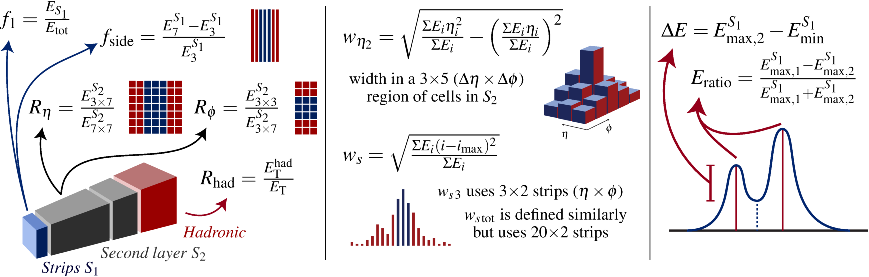
\includegraphics[width=\textwidth]{figures/photon_ID_variables.pdf}
  \caption{\label{fig:showerVars} Variables used to identify photon candidates which include quantities that summarize both the lateral and longitudinal (i.e., in depth) shower shape~\cite{atlascollaboration2023electron}. }
\end{figure}

Two domain-adaptation methods, which have already been applied in other contexts within HEP, will be studied in parallel. Initially, they will be applied to photon-energy calibration using the existing BDT energy regression, and subsequently with a more advanced approach that utilizes GNNs and low-level calorimeter information. The PI's team will apply the adversarial and distance correlation approaches studied by the PI on a simplified toy example using the existing BDT. The existing BDT, which has been extensively studied for various improvements, will serve as a benchmark to ensure that the domain-adaptation techniques do not negatively affect the original ML algorithm.

First, the PI's team, in collaboration with ATLAS $e/\gamma$ experts, will produce a simulation dataset modified to resemble actual data. This ``manipulated'' simulation will allow for more control over properties such as photon purity, energy scale, and sample size for initial studies; the team will also consider using recorded data during training once the domain-adaptation techniques reach a mature state. The team will use the previously developed toy model as a basis to develop domain-adaptation techniques for the energy regression BDT. As a former convener of the ATLAS Full Simulation group, which aims to improve both the physics and computational performance of the ATLAS detector simulation based on GEANT4~\cite{Agostinelli:2002hh}, the PI will also work with Full Simulation experts to better understand the sources of mismodelling.

The figure of merit for determining the best domain adaptation approach from the two more established methods will be the energy resolution. The framework developed to apply these methods will be carried over for use in more complex ML calibrations. The approach that results in the best physics performance, i.e., with the best energy resolution quantified by the lowest 50\% interquartile range, and with the best data-simulation agreement, will be chosen for further validation and integration into the ATLAS $e/\gamma$ photon calibration procedure. This improved energy calibration could then be used across \hyy\ measurements during the LHC Phase-II shutdown using the full Run~3 dataset."

A GNN-based photon-energy calibration is being developed by the University of Edinburgh, University of California at Berkeley, Lawrence Berkeley National Laboratory, and Michigan State University, and has shown promise in improving the photon energy resolution significantly (up to 20\%). However, the calibration resulting from the GNN-based approach differs for data and simulation. The PI's team with collaborate with the GNN calibration team to introduce domain-adaptation approaches to the powerful GNN calibration. This will be done after the distance correlation and adversarial techniques have been applied and tested on the simpler BDT-based calibration.  

The PI's team will use the toy data set to develop a domain adaptation approach which will extract features that are robust against simulation mismodelling using the toy manipulated-simulation dataset. This will be done using an autoencoder, which reduces the dimensionality of input features, that has an additional domain adaptation figure of merit during training. The domain-adaptation methods studied for the photon energy regression, i.e., distance correlation and adversarial networks, will be used to ensure that the encoded features are insensitive to data-simulation differences. The learned features could then be used for a variety of tasks, e.g., energy determination or object ID.

\paragraph{The deliverables for the photon-energy determination with domain adaptation work:}
\begin{itemize}
\item An improved BDT-based photon-energy calibration with up to a 15\% better resolution and similar performance in recorded and simulated data
\item Experience employing domain-adaptation techniques, i.e., distance correlation and adversarial networks, for calibration tasks within ATLAS
\item Further improved (up to 20\% over the BDT) photon-energy calibration that is robust against data-simulation differences
\item A new approach, feature representation transfer, that automatically produces features that are robust against data-simulation differences or other domain changes
\end{itemize}

\subsection{Enabling the Calibration of ML-based Photon ID with Domain Adaptation}

The ATLAS photon ID utilizes similar quantities to what are used for the photon-energy calibration, of which some are highlighted in Figure~\ref{fig:showerVars}. Unlike the photon-energy calibration, the ATLAS photon ID does not make use of a multivariate approach. This is due to the calibration procedure for the photon ID, which requires the ID algorithm to be independent of track isolation. This calibration procedure derives correction factors that adjust efficiencies derived from simulation to match efficiencies measured in data. The requirement for the ID algorithm to be independent from isolation comes from the procedure of measuring the efficiency in recorded data. The domain-adaptation techniques, that this proposal aims to prepare for calibration tasks, may be the key to moving the photon ID to a multivariate technique such as a BDT or approaches that use low-level variables such as GNNs. These multivariate approaches have been shown to improve the ID efficiency up to 10\% at a similar background rejection to the existing rectangular-requirement-based method. Once the move to multivariate methods is enabled by domain-adaptation techniques, these same approaches can then be extended to minimize the very data-simulation difference that the calibration procedure aims to correct.

The PI's team will work closely with photon reconstruction experts at Northern Illinois University (NIU) who have previously studied the use of BDTs and CNNs for photon identification, members of the ALCF data science group who have studied PointCloud~\cite{ATL-PHYS-PUB-2021-002} NNs for object ID to develop a multivariate photon ID method, and other ATLAS collaborators who have used ML approaches for photon ID. The domain-adaptation techniques will first be applied to a BDT or an NN that takes high-level quantities as inputs, similar to those currently used in the rectangular-requirements-based approach. As with the energy resolution calibration, both distance correlation and adversarial techniques will be studied in parallel by the two postdocs of the team. Once the output of the multivariate technique has been shown to be independent of the isolation, the team will work to fully calibrate the new ID algorithm together with collaborators at NIU (e.g., working with students who visit Argonne via the ATC or the Office of Science Graduate Student Research Program) using the standard techniques described in~\cite{PERF-2013-04,PERF-2017-02}.

The experience gained from applying the domain-adaptation techniques on a high-level inputs will then be used to apply similar methods to a GNN that uses low-level inputs i.e., energy deposits in the calorimeter cells.

Finally, the photon ID algorithm will be trained with manipulated simulation to make it more robust against mismodelling, as was done with the photon energy calibration. 

\paragraph{The following deliverables are expected from the proposed photon ID work:}
\begin{itemize}
\item An improved BDT- or NN-based photon ID algorithm that is independent from isolation and thus can be calibrated using existing techniques
\item A GNN-based photon ID algorithm that utilized more information than BDT/NN-based method and that inherently has the same behavior for both simulated and recorded data
\end{itemize}

\subsection{\hyy\ Differential Cross-Section Measurements with Decorrelated Background Estimations and Photon ID}
\begin{figure}[ht]
  \centering
  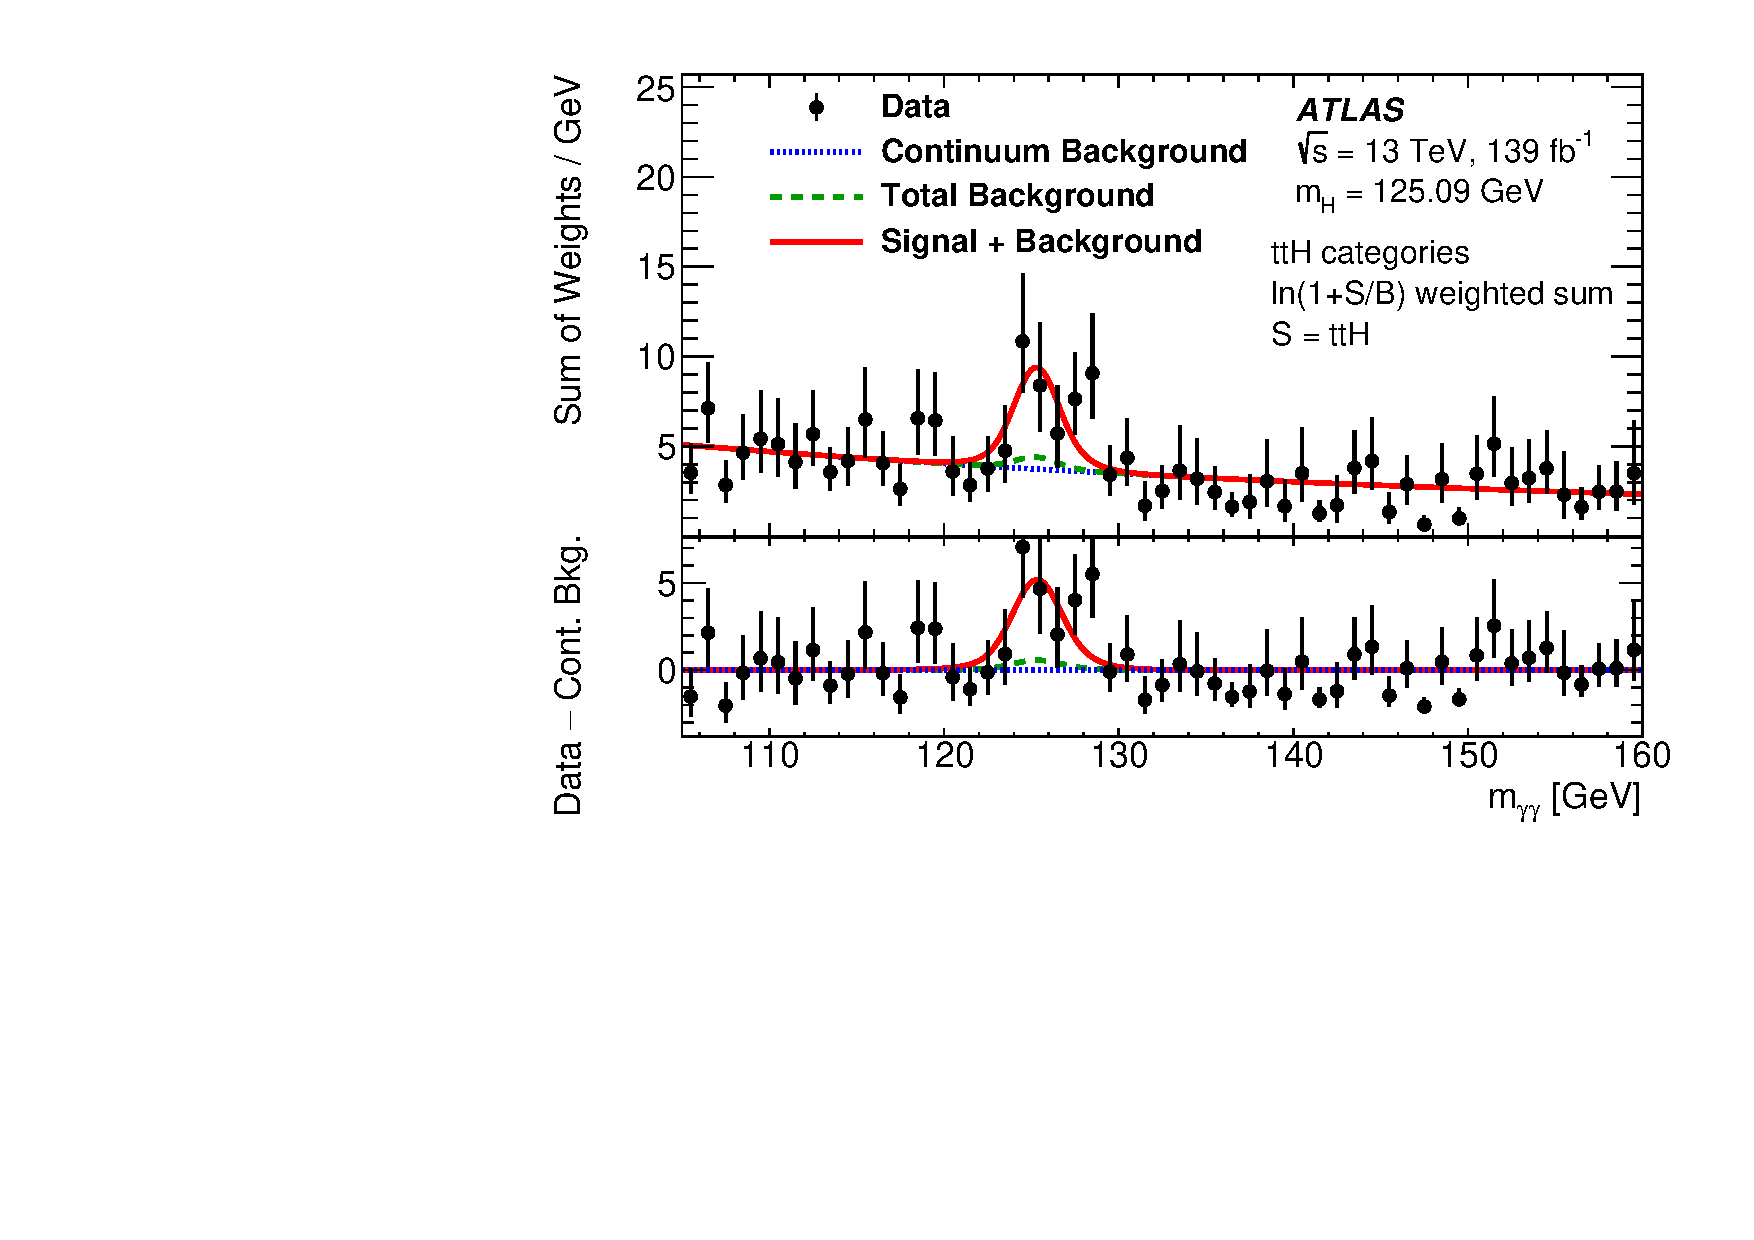
\includegraphics[width=0.6\textwidth]{figures/tth_myy.pdf}
  \caption{\label{fig:myy} Distribution of the diphoton invariant mass in the \ttH\ channel for the latest STXS ATLAS result~\cite{ATLAS_STXS}. The data (dots) are shown together with the sum of the fitted signal plus background (solid line). The blue dotted line represents the sum of the fitted continuum background, while the dashed line combines the contributions of continuum background and other Higgs boson events. The shape of the mass distribution must not be altered by the MVA which is used to discriminate background from signal. The domain-adaptation approaches proposed in this text can improve the discrimation power of MVAs while ensuring the MVA does not sculpt the \myy\ spectrum.}
\end{figure}

The most recent ATLAS results that performed many differential cross-section measurements in the \hyy\ channel made use of BDTs to both discriminate between the differential cross-section bins and to separate background from signal processes. One of the main backgrounds in many channels is the continuum diphoton background which is estimated using a functional fit to the \myy\ spectrum (see Figure~\ref{fig:myy} for an example). Due to this background estimation methodology, only variables that were found to have less than a 5\% linear correlation with the \myy\ spectrum were used in the BDT training. The domain-adaptation techniques used to improve the photon energy calibration can also be used to ensure that an ML classifier is independent of the \myy\ spectrum. This application of domain-adaptation approaches is similar to techniques that have been proposed to decorrelate algorithms to identify substructure within a jet from the mass of the jet, allowing the technique to be used for any mass of a hypothesised BSM particle.

The PI's team will contribute to the ``intermediate'' \hyy\ differential cross-section measurement which was initiated in early 2024 and will use a part of the Run~3 data. The team will focus on re-optimizing the BDTs trained to discriminate between the differential cross-section bins and between signal and the dominant background. This effort will familiarize the team with the existing ML strategy that does not incorporate domain adaptation to ensure that the BDTs are not correlated with the \myy\ spectrum.

Domain adaptation will be applied to the final Run~3 analysis that will use the full Run~3 dataset and that is expected to finalize near the end of the Phase-II shutdown. Using the framework that was developed for the photon ID MVA and energy calibration, the two postdocs and the PI will work in parallel to determine which domain adaptation approach, distance correlation vs adversarial vs feature representation transfer, is optimal for ensuring that the diphoton invariant mass spectrum remains uncorrelated with the signal-to-background MVA (either a BDT or NN). The method that both ensures that the background shape remains unchanged and results in the highest signal significance, which will now take advantage of more variables, will be used in the \hyy\ measurement.

In addition to using domain adaptation to ensure the stability of the \myy\ spectrum, the improved photon ID will be ready to be used in the final Run~3 \hyy\ measurement. The PI's team will focus on optimizing sensitivity to the \tthyy\ which is statistically limited and thus will especially benefit from the improved photon efficiency (reducing the statistical uncertainty by as much as 17\%).

\paragraph{The deliverables associated with the differential cross-section measurement are:}
\begin{itemize}
\item A publication describing the intermediate Run~3 \hyy\ measurement
\item A publication describing the final Run~3 \hyy\ measurement with improved photon ID and background rejection enabled by domain adaptation
\end{itemize}

\subsection{Integrating Domain Adaptation into an ML Framework}

Preparing certain domain adaptation approaches, such as developing adversarial models which can exhibit unstable training characteristics, can be technically challenging. Incorporating several techniques into a framework will not only ensure that physicists are more time-efficient when creating resilient ML models but will also allow for the exploration of various techniques, so that the most appropriate method can be chosen for a particular application. Domain-adaptation techniques will be explored and applied across various ML models (BDTs, NNs, and GNNs) and their applications, including object classification, property regression, and event classification. These models will be developed within the SALT framework, which is frequently used within ATLAS, to incorporate domain adaptation into a widely-used ML framework. SALT has already been employed, for example, to construct ML models for identifying boosted decays to two b-quarks, jets initiated by heavy flavor quarks, $\tau$-leptons, etc. Integrating features into SALT that allow ML models to be decorrelated from specific variables—such as data-simulation disparities, pile-up, and others—would reduce uncertainties and equip numerous algorithms for the demanding conditions of the HL-LHC.

Given that the photon ID, photon energy regression, and the \hyy\ signal-to-background ML models incorporating domain adaptation will be partially developed using SALT, the PI's team will have already integrated domain-adaptation techniques into SALT for specific implementations. This foundational work will facilitate the integration of a comprehensive domain adaptation framework into SALT. Common ML tasks, such as preprocessing of data (e.g., transforming input data to have ML-friendly numerical ranges), are already handled by the SALT environment. The domain-adaptation part of the framework will include the ability to use manipulated simulation data for preliminary testing of domain adaptation strategies and the application of various domain-adaptation methods. Finally, validation plots will be generated to illustrate any residual correlations, utilizing different techniques\cite{Shenoy_2023}. These will include distance correlation when using adversarial models, and the effectiveness of a discriminator trained to distinguish between domains when distance correlation is implemented.

Incorporating domain-adaptation techniques into SALT would improve existing ML models, such as those used for flavor tagging, and extend these benefits to new applications. This includes electron ID and energy determination, which naturally builds on the proposed work for photon ID and energy regression. Furthermore, these techniques could bolster the resilience of classifiers used for signal-to-background separation against experimental uncertainties like jet energy scale and resolution, thus improving physics measurements and searches across ATLAS. To aid in the adoption of the proposed framework within ATLAS, the PI will draw from his experience as one of the ATLAS ML forum conveners to co-organize tutorials at the annual ATLAS ML Forum Workshop that provide an introduction to domain adaptation and the proposed framework.

Beyond ATLAS, the proposed domain-adaptive framework has the potential to develop robust ML models for both current and future collider experiments as well as for a broad range of experiments across the HEP frontiers. The PI will engage with members of the Argonne HEP division, who work on a range of experiments including Mu2e, DUNE, and CMS-S4, to ensure there is across-frontier applicability of the proposed domain-adaptive framework.

The effort to include domain adaptation, which requires significant computing resources during the training of an ML model, into SALT will be supported by synergistic activities within the Argonne ATLAS group. These efforts are geared towards equipping SALT to utilize High-Performance Computing (HPC) systems, which are expected to drastically cut down training times (preliminary studies indicate a reduction from several days to just a few hours). Additionally, the PI is a co-lead for the High-Energy Physics Center for Computing Excellence (HEP-CCE) Scaling ML group. This group's goal is to facilitate the use of multinode HPCs for ML model development and thus will benefit the domain-adaptive framework. Leveraging the extensive computing capabilities of HPCs will ensure that the implementation of domain adaptation is not constrained by computational limitations.

The primary deliverable of this effort is the addition of domain adaptation methods, i.e., at least distance correlation and adversarial networks, into an existing ML framework (SALT) which can be used across ATLAS and HEP.
\clearpage
\subsection{Timetable of Activities}
\label{sec:timetable}
% https://lhc-commissioning.web.cern.ch/schedule/LHC-long-term.htm

The timetable of activities is shown in Figure~\ref{fig:timetable}.
\begin{figure}[!htbp]
  \centering
  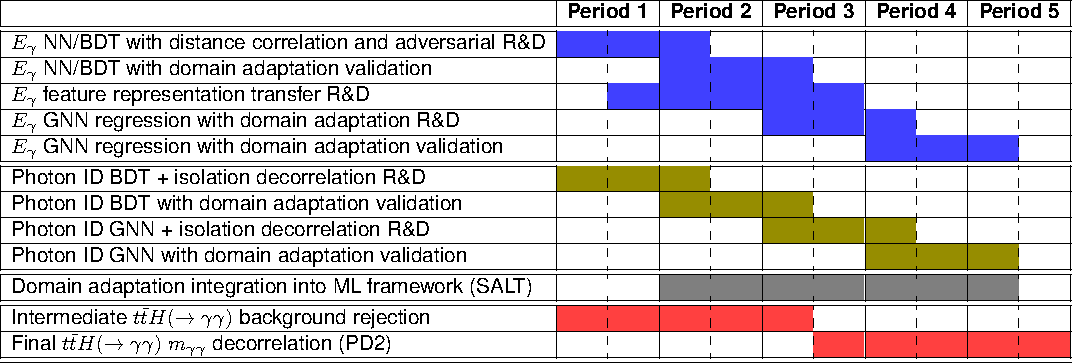
\includegraphics[width=\textwidth]{figures/timeline.pdf}
  \caption{Expected time spent on the work proposed in this text by the PI's team which will consists of two postdocs (at 1.0 FTE each) and about half of the PI's effort. Each period is 12 months long with Period 1 starting on August 1st 2024 and Period 5 ending on July 31st 2029 which is two months after the HL-LHC is slated to start operations (May 2029). The tasks include the application of domain adaptation  techniques to photon energy ($E_{\gamma}$) determination. Two established techniques will be studied, distance correlation and adversarial networks (AN), as well as a new technique, feature representation transfer. A subset of domain-adaptation techniques which decorrelate the ML model's output from certain features will be used for photon ID and signal-to-background separation in the $\ttbar H$ differential cross-section measurement.
  }
  \label{fig:timetable}
\end{figure}

Below is a summary of the milestones:
\begin{enumerate}
\item Reduction in photon energy resolution due to mitigation of data-simulation differences using domain adaptation.
\item Multivariate photon ID that is decorrelated from isolation
\item Updated intermediate \hyy\ differential cross-section measurement using part of the Run~3 dataset
\item Improved background rejection in \hyy\ enabled by domain adaptation being applied to decorrelate signal-to-background discriminating ML from the \myy\ spectrum
\item Integration of domain adaptation into ML framework (SALT) for broad use within ATLAS
\end{enumerate}

\subsection{Personnel and Resources}
\label{sec:personnel}
The PI will lead a team to execute the proposed project, involving an average of 2.0 postdoctoral FTEs and contributing 50\% of the PI's effort. These postdocs, fully funded by this award, are slated to begin at the start of the first and second budget periods and will continue through the fifth budget period. Their responsibilities will be divided between implementing domain adaptation strategies and conducting two differential cross-section measurements in the \hyy\ channel. One postdoc will gain expertise in photon energy determination while the other postdoc will work on photon ID using the same ML domain-adaptation methods. Both postdocs will contribute to developing feature representation transfer and will work on preparing the next two iterations of the \hyy\ differential cross-section measurement.
% Add a table showing who will work on what

% \begin{table}
%   \caption{\label{tab:personnel}}
%   \begin{tabular}{|l|c|c|c|c|} \hline
%     & {\textbf PI} & {\textbf Postdoc 1} & {\textbf Postdoc 2} & {\textbf Student} \\  \hline\hline 
%     Adversarial & used & complex correlations & high \\ \hline
%     Distance Correlation & used & non-linear correlations & low \\ \hline
%     Feature Transfer & not used & features for multiple tasks  & medium \\ \hline\hline                                                                                                                                       
%   \end{tabular}
% \end{table}
Additionally, the PI will engage with graduate and undergraduate students on this research through established connections with local universities, supported by several programs. The PI has a track record of mentoring students who participate in programs such as the DOE Office of Science Graduate Student Research program and the Science Undergraduate Laboratory Internships. Furthermore, the Argonne ATLAS Center, which welcomes graduate students from ATLAS collaboration member universities, offers further collaborative opportunities. The PI will work with students from institutions that have existing ties with the Argonne ATLAS group, including NIU, which boasts expertise in photon and Higgs sectors and runs a computing traineeship~\cite{C2THEP2} aligning with the computational demands (i.e., the infrastructure needed for the framework) of this proposal.
% Need to be specific about what I will be doing
For computing needs, the PI will access resources at the Argonne through the Laboratory Computing Resources Center (LCRC), which boasts a significant setup (825 nodes, each with 128 cores) frequently utilized by the Argonne ATLAS group and ATLAS Analysis Center (ATC) university collaborators for preparing ATLAS measurements for publication. Additionally, the PI will use a specialized system at LCRC, comprising six nodes with eight GPUs each, for ML model development. The Argonne ATLAS group holds a renewable computing allocation at LCRC, which can be expanded as required for the proposed tasks. The Argonne Leadership Computing Facility (ALCF) provides further resources and expertise, including both NVIDIA and Intel GPU capabilities, to support the development and training of complex ML models. The PI's team will leverage existing relationships with ALCF experts to develop and refine domain-adaptation approaches, crucial to computing scientists, using ALCF resources. Requests for resource allocations will be made as needed to support these activities.


\section{Summary}
Machine learning has become an indispensable tool in HEP, enhancing capabilities in tasks such as particle identification and distinguishing between signal and background processes. However, as we approach the era of the HL-LHC with its unprecedented data scale, ML models must become more robust to effectively mitigate the impact of systematic uncertainties on physics measurements. Domain-adaptation approaches have shown potential in reducing these uncertainties and improving the robustness of models against experimental conditions and data-simulation discrepancies. This proposal outlines the integration of domain-adaptation techniques into an ML framework to make these methods broadly accessible, thus potentially impacting a wide range of HEP measurements. This effort is crucial for future discoveries in collider physics, especially in the precision era of the HL-LHC, where precise measurements are key to probing the effects of BSM physics.
\clearpage

\appendix
\renewcommand{\thesection}{\arabic{section}} % Reset numbering with Arabic numbers
% Apply custom format to section titles in appendices
\titleformat{\section}
  {\normalfont\Large\bfseries}{Appendix \thesection:}{1em}{}
\addcontentsline{toc}{part}{Appendices}

\printbibliography[title={Bibliography and References},heading=bibnumbered]
\clearpage

\section{Facilities and  other resources}
Argonne offers various resources, including office space for postdocs and potential students as well as several computing resources. The computing resources expected to be utilized include CPU and GPU resources available through the Laboratory Computing Resource Center at Argonne. These resources are expected to be used to produce input data for ML algorithms as well as training the ML algorithms. The PI also plans to use computing resources at the ALCF resources, such as Polaris (which has NVIDIA GPUs) and Aurora (which contains Intel GPUs), via a discretionary allocation. These resources will be used for large-scale training and optimization of the proposed approach.

An additional important resource is the ATLAS experiment at the LHC at CERN. The PI's team will make use of ATLAS data and simulation for the proposed studies and will occasionally travel to CERN to work with international collaborators.

\clearpage

\section{Equipment}
The requested funding will be used to purchase two laptops for the postdocs that the PI will supervise. The combined cost of the three laptops is expected to be \$6,418.

\clearpage

\section{Data management plan}
The majority of the data and code produced will come from the ATLAS experiment. ATLAS has its own data management plan which the PI's team will adhere to; the details of that plan can be found at \url{https://po.usatlas.bnl.gov/programoffice/datamanagementpolicy.php}.

Scientific results that used ATLAS data will be published in a scientific journal or an ATLAS publication note, which will be publicly available on \url{https://arxiv.org/} and \url{https://twiki.cern.ch/twiki/bin/view/AtlasPublic/SimulationPublicResults}, respectively. Figures and tables will be made available in the same way as other ATLAS results, via HEPData (\url{https://www.hepdata.net/}) and ATLAS public pages. 

Additional data that are produced outside of ATLAS for initial ML algorithm development will be stored on the Argonne High Energy Physics divisional nodes in the HDF5 format and will consist of energy deposits in a simplified detector. The generated data are expected to occupy a small fraction of the available data storage on these nodes. Code and configurations used for the development of the algorithm and production of data will be kept at the Argonne Computing, Environment and Life Sciences (CELS) gitlab repository: \url{https://xgitlab.cels.anl.gov/}. Results from these studies, if published, will be publicly available on \url{https://arxiv.org/}. 

\clearpage

\section{Promoting Inclusive and Equitable Research (PIER) Plan}

Achieving and maintaining long-term success requires the creation of a safe and welcoming environment that fosters diversity, equity, and inclusion (DEI). An environment that promotes DEI will enhance the proposed research by nurturing creativity in problem-solving and by encouraging constructive criticism from individuals with diverse backgrounds and perspectives. This appendix summarizes the key aspects of how the PI will approach DEI for the proposed work within the ATLAS group and the HEP division at Argonne, as well as how the PI plans to improve DEI.

The PI will ensure an inclusive and equitable work environment. All personnel, including two postdocs hired for this proposal and any students and postdocs from collaborating institutions, will be encouraged to express their ideas in an environment that promotes curiosity and openness. This will be facilitated through both semi-formal and formal settings. Formal idea exchanges will include group meetings with collaborators, where members of the working group are encouraged to ask questions or suggest improvements to the proposed work. Topics will be discussed among all involved personnel to foster leadership on a subtopic by postdocs and students. Additionally, postdocs will be assigned a mentor outside the ATLAS group, in accordance with HEP division policy, who will discuss career goals from a non-ATLAS perspective.

The PI will also meet individually with group members at least once a week to discuss ideas for the proposed work. These meetings are intended to build the confidence of junior postdocs and students, enabling them to express ideas and provide constructive feedback both within and outside the group.

\subsection{How This Work Will Enhance DEI}

The PI is committed to fostering opportunities and removing obstacles for those on the path to becoming career scientists. Outreach programs are instrumental in enlarging the candidate pool, particularly for underrepresented minorities (URMs). Drawing from previous outreach experience, the PI will illuminate the diverse career paths available to students who pursue advanced degrees in HEP, both within academia and beyond. It is often overlooked that qualifications in HEP can lead to fulfilling careers outside the field, particularly in industries that value expertise in ML and computing. During outreach activities, the PI will emphasize the broad spectrum of career opportunities that ML and computing skills can unlock.

To further support these efforts, the PI will recruit undergraduate students for proposed projects through various summer initiatives. The USATLAS Summer Undergraduate Program for Exceptional Researchers (SUPER), sponsored by USATLAS, provides financial assistance to exceptional undergraduates in the US for summer research in areas like ATLAS physics analysis and computing. Expanded in 2022, SUPER now includes students from non-USATLAS minority-serving institutions (MSIs). Additionally, the PI will continue recruiting through the Science Undergraduate Laboratory Internships (SULI) and participating in the Look@Argonne event, which promotes internship opportunities at Argonne to Louis Stokes Alliances for Minority Participation affiliated institutions, highlighting the ATLAS group’s opportunities through panel discussions.

The PI has also been instrumental in leading traineeship programs that mentor early-stage researchers. Alongside USATLAS universities, the PI co-organized the CAMPFIRE events in 2019, 2022, and 2023, which are designed to build a supportive and inclusive community of USATLAS graduate students. These events, featuring educational, technical, and social activities, strive to foster connections among students from historically underrepresented groups, addressing potential feelings of isolation they might encounter at their home institutions or at CERN, and preparing them for future stages of their careers.

In addition to engaging with graduate students through traineeship programs, the PI has hosted graduate students from collaborating universities via the USATLAS ATLAS Center (ATC) and the Office of Science Graduate Student Research (SCGSR) Program. The PI plans to deepen these collaborations, actively involving more graduate students at Argonne in the proposed projects. This integration not only provides graduate students with experience working at a national laboratory on ML projects but also contributes valuable insights and efforts to the research.

In hiring practices, the PI adheres to the best practices of the Argonne HEP division, which include advertising positions directly to MSIs and ensuring that selection committees, often led by a chair who has completed bias training from the Argonne Human Resources department, are aware of implicit biases. The PI also implements a co-developed strategy within the ATLAS group that includes blind reviews of candidates to prevent groupthink and bias, enhancing the fairness and inclusivity of the hiring process.
% Add committee member info

\subsection{Conclusion}

The PI is dedicated to cultivating a research environment that not only supports but also thrives on DEI. Central to these efforts is the development of a work culture that welcomes input from all members, nurturing leadership skills among postdocs and students, and facilitating their involvement in high-impact research topics. Moreover, the PI's proactive approach to expanding the diversity of the research pool—through targeted recruitment from minority-serving institutions and outreach initiatives—highlights a strategic commitment to accessibility and representation in science. The PI's leadership in events like the CAMPFIRE traineeship programs further exemplifies a commitment to mentorship and the development of an inclusive community of physicists. Finally, adherence to equitable hiring practices, including bias training and blind review processes, underscores a systematic approach to fostering an inclusive research environment.

\clearpage

\section{Other attachments}
There are no other attachments.

\end{document}
